% Part I: the projection-based controller.
% Sources: THEORY_REVISED.md Sections 1-5 and 7; ASSESSMENT.md Sections 2 and 4; results/factorial/table.md,
% results/comparison_complete_table.md, results/fair_n1/table.md, results/oracle_ruub/table.md,
% results/monte_carlo_honest/summary.md.

% =====================================================================================================================
\section{Setting and standing assumptions}\label{sec:p1-setting}

This part replaces the stability argument of version~1 with a statement whose assumptions are explicit, whose
algorithm is exactly the one in \code{src/core/} of the accompanying repository, and whose every step is either proved
here or verified numerically by \code{tests/test_theorem_to_code.py}. The errata to version~1 are listed in
Section~\ref{sec:version1}; Section~\ref{sec:p1-prior} positions the result against prior work.

\paragraph{Notation.} $\norm{\cdot}$ is the Euclidean norm for vectors and the Frobenius norm for matrices;
$\operatorname{vec}(\cdot)$ is the row-major vectorisation used throughout the code; there are $m$ kernels and $n$
states.

\paragraph{Plant, reference and error.}
\begin{gather}
\dot x = f(x,t)+u,\qquad e = x-x_m(t),\qquad u = \dot x_m-k_e e-\fhat(x),\label{eq:part1:plant}\\
\fhat(x) = W^\T\varphi(x,c,\sigma),\qquad
\varphi_i(x) = \exp\Bigl(-\frac{\norm{x-c_i}^2}{2\sigma_i^2}\Bigr).\label{eq:part1:network}
\end{gather}

\begin{rmk}{Assumption}{A1}[operation on a compact set]
There is a compact set $X\subset\R^n$ with $x(t)\in X$ for all $t\ge0$, and
$F_{\max}:=\sup_{x\in X,\,t\ge0}\norm{f(x,t)}<\infty$.
\emph{(Version~1 assumes ``a compact spatial domain $X$'' in the same way. For globally bounded $f$ the assumption is
discharged by Theorem~1(iv); for the Lorenz plant it is a genuine assumption.)}
\end{rmk}

\begin{rmk}{Assumption}{A2}[reference]
$x_m$ is $C^1$ with $x_m$, $\dot x_m$ bounded, and $\dot x_m$ is available to the controller.
\end{rmk}

\begin{rmk}{Assumption}{A3}[admissible ideal parameters]
There is a curve $\theta^*(t)=(W^*(t),c^*(t),\sigma^*(t))$ lying for all $t$ in the \emph{inner} projection sets
\[
\norm{W^*}\le W_{\max}-\varepsilon,\qquad \norm{c^*}\le c_{\max}-\varepsilon,\qquad
\sigma_{\min}+\varepsilon\le\sigma^*_i\le\sigma_{\max}-\varepsilon.
\]
\end{rmk}

\begin{rmk}{Assumption}{A4}[ideal-parameter regularity]
$\theta^*(\cdot)$ is $C^1$ with $\norm{\dot W^*}\le V_W$, $\norm{\dot c^*}\le V_c$, $\norm{\dot\sigma^*}\le V_\sigma$.
(For a time-invariant plant one may take $\theta^*$ constant, $V_W=V_c=V_\sigma=0$.)
\end{rmk}

\begin{rmk}{Assumption}{A5}[gains and geometry]
$k_e>0$; $\Gamma_W$, $\Gamma_c$ symmetric positive definite on $\R^{mn}$ (a zero $\Gamma$ freezes that group, see
Remark~3); $\Gamma_\sigma$ diagonal positive; $0<\varepsilon<\min\bigl(W_{\max},\,c_{\max},\,(\sigma_{\max}-\sigma_{\min})/2\bigr)$;
$\sigma_{\min}>0$.
\end{rmk}

\paragraph{Remarks on the assumptions.}
\begin{itemize}
\item \textbf{The proof never uses optimality of $\theta^*$.} $\theta^*$ is an analytic device; any admissible $C^1$
  curve works, and the approximation quality of the network enters the result only through the \emph{actual} size of
  the disturbance $d(t)$ defined below, not through the bound. The Tikhonov-regularised definition of $\theta^*$ in
  version~1 and its implicit-function-theorem (IFT) argument for A4 are therefore unnecessary --- and, as written, not a
  proof (erratum E3, Section~\ref{sec:version1}).
\item \textbf{No centre-separation constraint is needed.} The set $\{c:\norm{c_i-c_j}\ge\delta\ \forall\, i\ne j\}$ is
  not convex, so no projection onto it has property (P) below; the claim of version~1 that separation is ``maintained
  via the projection set construction'' is withdrawn (erratum E1, Section~\ref{sec:version1}). The bounded-Jacobian
  property that the proof needs follows from $\sigma\ge\sigma_{\min}$ alone.
\end{itemize}

% =====================================================================================================================
\section{The algorithm}\label{sec:p1-algorithm}

The algorithm is identical to the one implemented in \code{src/core/controller.py}:
\begin{equation}\label{eq:part1:laws}
\begin{aligned}
\dot W &= \operatorname{Proj}_W\bigl(W,\ \Gamma_W\,\varphi e^\T\bigr),\\
\dot c &= \operatorname{Proj}_c\bigl(c,\ \Gamma_c\,\varphi_c'^{\T}We\bigr),\\
\dot\sigma &= \operatorname{Proj}_\sigma\bigl(\sigma,\ \Gamma_\sigma\,\varphi_\sigma'^{\T}We\bigr),
\end{aligned}
\end{equation}
with $\varphi'_c=\partial\varphi/\partial\operatorname{vec}(c)\in\R^{m\times mn}$ (row $i$ has the single non-zero
block $\varphi_i(x-c_i)^\T/\sigma_i^2$) and $\varphi'_\sigma=\operatorname{diag}\bigl(\varphi_i\norm{x-c_i}^2/\sigma_i^3\bigr)$.

\paragraph{Norm-ball projection ($W$ and $c$), boundary layer of width $\varepsilon$.}
\begin{equation}\label{eq:part1:proj}
\operatorname{Proj}(\theta,\Gamma y)=
\begin{cases}
\Gamma y-h(\theta)\,\Gamma\theta\,\dfrac{\theta^\T\Gamma y}{\theta^\T\Gamma\theta}
  & \text{if } h(\theta)>0 \text{ and } \theta^\T\Gamma y>0,\\[8pt]
\Gamma y & \text{otherwise},
\end{cases}
\end{equation}
\begin{equation}\label{eq:part1:h}
h(\theta)=
\begin{cases}
0 & \text{for } \norm{\theta}\le\theta_{\max}-\varepsilon,\\
\bigl((\norm{\theta}-\theta_{\max}+\varepsilon)/\varepsilon\bigr)^2 & \text{in between},\\
1 & \text{for } \norm{\theta}\ge\theta_{\max}.
\end{cases}
\end{equation}

\paragraph{Box projection ($\sigma$, component-wise).} The update component is multiplied by
$\clip\bigl((\sigma_i-\sigma_{\min})/\varepsilon,0,1\bigr)$ when it points below the lower face and by
$\clip\bigl((\sigma_{\max}-\sigma_i)/\varepsilon,0,1\bigr)$ when it points above the upper face.

\paragraph{Discrete time.} The simulations integrate with fixed-step RK4 and re-clip the parameters to their sets after
every stage (\code{src/core/integrator.py}). The theorem is a continuous-time statement; the clip is a safety net that
is inactive if the step is small enough (property (P) already removes the outward component on the boundary).

% =====================================================================================================================
\section{Lemmas and the boundedness theorem}\label{sec:p1-theorem}

\subsection{Lemmas}

\begin{thm}{Lemma}{1}[projection property (P)]
Under A3 and A5, for every $\theta$ in its set and every $y$,
\begin{equation}
\tilde\theta^\T\Gamma^{-1}\operatorname{Proj}(\theta,\Gamma y)\le\tilde\theta^\T y,
\qquad \tilde\theta:=\theta-\theta^*. \tag{P}
\end{equation}
\end{thm}

\begin{proof}
If the projection is inactive the two sides are equal. Otherwise
\[
\tilde\theta^\T\Gamma^{-1}\bigl(\operatorname{Proj}{}-\Gamma y\bigr)
=-h\,\frac{\theta^\T\Gamma y}{\theta^\T\Gamma\theta}\,\tilde\theta^\T\theta,
\]
with $h>0$ and $\theta^\T\Gamma y>0$, and
$\tilde\theta^\T\theta=\norm{\theta}^2-\theta^{*\T}\theta\ge\norm{\theta}\bigl(\norm{\theta}-\norm{\theta^*}\bigr)\ge0$
because $h>0$ forces $\norm{\theta}\ge\theta_{\max}-\varepsilon\ge\norm{\theta^*}$. For the box, component $i$, with
$s_i$ the clip factor applied to that component: $\tilde\sigma_i(s_i-1)y_i\le0$ because $s_i\le1$, and on the lower
face $y_i<0$ while $\tilde\sigma_i=\sigma_i-\sigma^*_i\le\sigma_{\min}+\varepsilon-\sigma^*_i\le0$ (symmetrically on
the upper face).
\end{proof}
\status{Proved.}
\checkedby{\code{tests/test_projection.py} (randomised; isotropic and non-isotropic $\Gamma$; vector, matrix and box),
together with the counterexample showing that (P) fails when $\theta^*$ is outside the inner set.}

\begin{thm}{Lemma}{2}[lumped disturbance]
Define
\begin{equation}\label{eq:part1:d}
d:=f-\fhat+\tilde W^\T\varphi+W^\T\varphi'_c\,\tilde c+W^\T\varphi'_\sigma\,\tilde\sigma.
\end{equation}
Then identically
\begin{equation}\label{eq:part1:edot}
\dot e=-k_e e-\tilde W^\T\varphi-W^\T\varphi'_c\,\tilde c-W^\T\varphi'_\sigma\,\tilde\sigma+d,
\end{equation}
and under A1, A3,
\begin{gather}
\norm{d}\le D_{\max}:=F_{\max}+3W_{\max}\sqrt m
  +W_{\max}\bigl(2c_{\max}J_c+\sqrt m\,(\sigma_{\max}-\sigma_{\min})J_\sigma\bigr),\label{eq:part1:Dmax}\\
J_c=\mathrm{e}^{-1/2}/\sigma_{\min},\qquad J_\sigma=2\mathrm{e}^{-1}/\sigma_{\min}.\notag
\end{gather}
\end{thm}

\begin{proof}
The identity is the definition of $d$ substituted into $\dot e=-k_e e+f-\fhat$. For the bound: $\norm{f}\le F_{\max}$;
$\norm{\fhat}\le\norm{W}\norm{\varphi}\le W_{\max}\sqrt m$ ($0<\varphi_i\le1$); $\norm{\tilde W}\le2W_{\max}$;
$\norm{\tilde c}\le2c_{\max}$; $\norm{\tilde\sigma}\le\sqrt m\,(\sigma_{\max}-\sigma_{\min})$; the rows of $\varphi'_c$
have disjoint supports, so
\[
\norm{\varphi'_c}_2=\max_i\frac{\varphi_i\norm{x-c_i}}{\sigma_i^2}
\le\sup_{r\ge0}\frac{r\,\mathrm{e}^{-r^2/(2\sigma^2)}}{\sigma^2}=\frac{\mathrm{e}^{-1/2}}{\sigma}\le J_c,
\]
and $\norm{\varphi'_\sigma}_2=\max_i\varphi_i\norm{x-c_i}^2/\sigma_i^3\le2\mathrm{e}^{-1}/\sigma\le J_\sigma$.
\end{proof}
\status{Proved.}
\checkedby{\code{tests/test_rbf_kernel.py} checks the two suprema by brute force.}

\begin{rmk}{Remark}{1}[local form]
Writing $\varphi^*=\varphi(x;c^*,\sigma^*)$ and expanding to first order in $(\tilde c,\tilde\sigma)$ gives
\[
d=\varepsilon+W^{*\T}O_{\mathrm{ho}}+\tilde W^\T\varphi'_c\,\tilde c+\tilde W^\T\varphi'_\sigma\,\tilde\sigma,
\qquad \varepsilon:=f-W^{*\T}\varphi^*,
\]
with $O_{\mathrm{ho}}$ the Taylor remainder --- the decomposition of version~1. Near convergence
($\tilde\theta\to0$) this shows $\norm{d}\lesssim\norm{\varepsilon}+O(\norm{\tilde\theta}^2)$, which is why the
controller performs far better than $D_{\max}$ suggests; but it does not yield a smaller global constant than Lemma~2,
which needs no Hessian and no Taylor expansion.
\end{rmk}

\begin{thm}{Lemma}{3}[Lyapunov derivative]
Let
\[
V=\tfrac12e^\T e+\tfrac12\operatorname{vec}(\tilde W)^\T\Gamma_W^{-1}\operatorname{vec}(\tilde W)
+\tfrac12\tilde c^\T\Gamma_c^{-1}\tilde c+\tfrac12\tilde\sigma^\T\Gamma_\sigma^{-1}\tilde\sigma.
\]
Along trajectories of the algorithm,
\begin{align}
\dot V&=-k_e\norm{e}^2+e^\T d+\mathrm{cross}-\Omega^*,\label{eq:part1:Vdot}\\
\mathrm{cross}&=\ip{\tilde W}{\Gamma_W^{-1}\dot W-\varphi e^\T}
  +\tilde c^\T\bigl(\Gamma_c^{-1}\dot c-\varphi_c'^{\T}We\bigr)
  +\tilde\sigma^\T\bigl(\Gamma_\sigma^{-1}\dot\sigma-\varphi_\sigma'^{\T}We\bigr)\le0,\notag\\
\Omega^*&=\ip{\tilde W}{\Gamma_W^{-1}\dot W^*}+\tilde c^\T\Gamma_c^{-1}\dot c^*
  +\tilde\sigma^\T\Gamma_\sigma^{-1}\dot\sigma^*,\qquad \abs{\Omega^*}\le C_\Omega,\notag\\
C_\Omega&:=2W_{\max}\norm{\Gamma_W^{-1}}_2V_W+2c_{\max}\norm{\Gamma_c^{-1}}_2V_c
  +\sqrt m\,(\sigma_{\max}-\sigma_{\min})\norm{\Gamma_\sigma^{-1}}_2V_\sigma.\notag
\end{align}
\end{thm}

\begin{proof}
Differentiate $V$, substitute the identity of Lemma~2 for $\dot e$, and use
$e^\T\tilde W^\T\varphi=\ip{\tilde W}{\varphi e^\T}$, $e^\T W^\T\varphi'_c\,\tilde c=\tilde c^\T\varphi_c'^{\T}We$,
$e^\T W^\T\varphi'_\sigma\,\tilde\sigma=\tilde\sigma^\T\varphi_\sigma'^{\T}We$. That $\mathrm{cross}\le0$ is Lemma~1
applied to the three groups; the bound on $\Omega^*$ is Cauchy--Schwarz with A3, A4.
\end{proof}
\status{Proved.}
\checkedby{\code{tests/test_theorem_to_code.py}: the identity (to machine precision) and $\mathrm{cross}\le0$ (at every
sample) are verified along simulated trajectories, on a plant that is exactly representable with known constant
$\theta^*$.}

\subsection{Theorem 1: uniform ultimate boundedness}

\begin{thm}{Theorem}{1}[uniform ultimate boundedness]
Assume A1--A5, let
\[
R_{\mathrm{UUB}}:=\frac{D_{\max}}{2k_e}+\sqrt{\frac{D_{\max}^2}{4k_e^2}+\frac{C_\Omega}{k_e}},
\]
and let $V_{\max,\Theta}$ be the supremum over the projection sets of the parameter part of $V$.
\begin{enumerate}[label=(\roman*)]
\item \textbf{Descent outside a ball.} $\dot V\le-k_e\norm{e}^2+D_{\max}\norm{e}+C_\Omega$, hence $\dot V<0$ whenever
  $\norm{e}>R_{\mathrm{UUB}}$.
\item \textbf{Pointwise ultimate bound.} Every solution satisfies $V(t)\le\max\{V(0),c_{\inf}\}$ with
  $c_{\inf}:=\tfrac12R_{\mathrm{UUB}}^2+V_{\max,\Theta}$, every level $c>c_{\inf}$ is reached in finite time, and
  \[
  \limsup_{t\to\infty}\norm{e(t)}\le\sqrt{R_{\mathrm{UUB}}^2+2V_{\max,\Theta}}.
  \]
\item \textbf{RMS bound (the quantitatively meaningful one).} For every $T_1<T_2$,
  \[
  \RMS_{[T_1,T_2]}(\norm{e})\le\frac{D_{\max}}{2k_e}
  +\sqrt{\frac{D_{\max}^2}{4k_e^2}+\frac{C_\Omega}{k_e}+\frac{V(T_1)}{k_e(T_2-T_1)}},
  \]
  so $\limsup_{T_2\to\infty}\RMS_{[T_1,T_2]}(\norm{e})\le R_{\mathrm{UUB}}$ --- \emph{without} the parameter-energy
  term of (ii). The same inequality holds with $D_{\max}$ and $C_\Omega$ replaced by the trajectory-wise suprema of
  $\norm{d(t)}$ and $\abs{\Omega^*(t)}$ on $[T_1,T_2]$.
\item \textbf{Reference bound (adaptation-free).} Under A1 and the hard parameter bounds alone,
  $\dot e=-k_e e+(f-\fhat)$ with $\norm{f-\fhat}\le F_{\max}+W_{\max}\sqrt m=:\tilde F$, so
  \[
  \norm{e(t)}\le\mathrm{e}^{-k_e t}\norm{e(0)}+\tilde F/k_e\qquad\text{for all }t,
  \]
  whatever the adaptation does.
\end{enumerate}
\end{thm}

\begin{proof}
\begin{enumerate}[label=(\roman*)]
\item Lemma~3 with Cauchy--Schwarz on $e^\T d$.
\item If $V>c_{\inf}$ then, since the parameter part of $V$ is at most $V_{\max,\Theta}$,
  $\tfrac12\norm{e}^2>\tfrac12R_{\mathrm{UUB}}^2$, so $\norm{e}>R_{\mathrm{UUB}}$ and $\dot V<0$; more precisely, with
  $\Delta:=V-c_{\inf}>0$ one has $\norm{e}^2\ge R_{\mathrm{UUB}}^2+2\Delta$ and therefore
  \[
  \dot V\le-g\Bigl(\sqrt{R_{\mathrm{UUB}}^2+2\Delta}\Bigr)=:-\psi(\Delta),\qquad g(r)=k_er^2-D_{\max}r-C_\Omega,
  \]
  with $g$ increasing for $r\ge R_{\mathrm{UUB}}$ and $\psi$ of class $\mathcal K$. The comparison lemma gives
  $V(t)\le\max\{V(0),c_{\inf}\}$, finite-time entry into every sublevel set $\{V\le c\}$ with $c>c_{\inf}$, and
  $\limsup V\le c_{\inf}$, i.e.\ the stated bound on $\norm{e}$ ($\norm{e}^2\le2V$).
\item Integrate (i):
  \begin{multline*}
  k_e\int_{T_1}^{T_2}\norm{e}^2\dd t\le V(T_1)-V(T_2)+D_{\max}\int_{T_1}^{T_2}\norm{e}\dd t+C_\Omega(T_2-T_1)\\
  \le V(T_1)+D_{\max}\sqrt{T_2-T_1}\,\sqrt{\int_{T_1}^{T_2}\norm{e}^2\dd t}+C_\Omega(T_2-T_1)
  \end{multline*}
  by Cauchy--Schwarz; with $S:=\RMS_{[T_1,T_2]}(\norm{e})$ this reads
  \[
  k_eS^2-D_{\max}S-\bigl(C_\Omega+V(T_1)/(T_2-T_1)\bigr)\le0,
  \]
  and $S$ is below the positive root.
\item Variation of constants.\qedhere
\end{enumerate}
\end{proof}
\status{Proved.}

\paragraph{What (ii)--(iv) say together.} Part (ii) is the conclusion of version~1; it is the textbook level-set
argument (Khalil~\cite[Thm.~4.18]{khalil2002}; Lewis et al.~\cite{lewis1999}) and its radius contains the
parameter-energy reservoir $V_{\max,\Theta}$ --- a bias-like term --- so it does \textbf{not} establish that
projection yields a tighter tracking bound than $\sigma$-modification. Part (iii) is tighter and is the statement
that can be checked without unknown constants: replace $D_{\max}$ by the measured $\sup\norm{d}$, see
\code{experiments/exp_oracle_ruub.py}, where it is satisfied in 48/48 runs (Section~\ref{sec:p1-experiments}).
Part (iv) shows that mere boundedness of $e$ is already a consequence of projection plus a stable error channel,
independent of the adaptation law; the content of adaptive control is in making the \emph{actual} $d(t)$ small, which
no a-priori constant captures. In the oracle experiments the a-priori $R_{\mathrm{UUB}}$ exceeds the observed RMS error
by factors of $915$ to $10954$.

\begin{rmk}{Remark}{2}[no LaSalle / Barbalat]
Version~1's claim that the argument needs neither LaSalle's invariance principle nor Barbalat's lemma is correct, and
standard: UUB statements never need them. Nothing here claims asymptotic convergence of $e$ or of $\tilde\theta$.
\end{rmk}

\begin{rmk}{Remark}{3}[frozen groups]
If $\Gamma_c=0$ (fixed centres), drop the $\tilde c$ term from $V$; the identity of Lemma~2 still holds with
$-W^\T\varphi'_c\,\tilde c$ absorbed into $d$, with the same bound. Likewise for $\sigma$.
\end{rmk}

\begin{rmk}{Remark}{4}[what is not proved]
Parameter convergence (it requires persistent excitation of a nonlinear-in-parameter regressor --- not addressed);
exact tracking; any statement about the size of the ideal approximation error $\varepsilon$.
\end{rmk}

% =====================================================================================================================
\section{The no-bias claim, stated precisely}\label{sec:p1-nobias}

With $\sigma$-modification,
\[
\dot V\le-k_e\norm{e}^2-\tfrac12\sigma_{\mathrm{mod}}\norm{\tilde\theta}_\Gamma^2
+\tfrac12\sigma_{\mathrm{mod}}\norm{\theta^*}_\Gamma^2+D\norm{e}+C_\Omega\text{:}
\]
the leak adds a positive constant and removes the parameter-energy reservoir, which gives exponential convergence of $V$
to a ball whose radius grows with $\sigma_{\mathrm{mod}}\norm{\theta^*}^2$. With projection,
\[
\dot V\le-k_e\norm{e}^2+D\norm{e}+C_\Omega\text{:}
\]
no positive constant is added, but nothing dissipates parameter energy, which is why the pointwise bound (ii) of
Theorem~1 keeps $V_{\max,\Theta}$. Projection therefore removes the \emph{Lyapunov-derivative} bias of leakage (true,
and known since Pomet--Praly~\cite{pp1992} and Ioannou--Sun~\cite{ioannou1996}), not the dependence of the ultimate
\emph{tracking} bound on the parameter set (false as stated in Sections~7.3 and~10.3 of version~1). Empirically the two
mechanisms are compared on identical geometry in \code{experiments/exp_bias_factorial.py}
(Section~\ref{sec:p1-experiments}).

% =====================================================================================================================
\section{Prior art}\label{sec:p1-prior}

\begin{itemize}
\item Adaptive Gaussian-network control with robust modification: Sanner and Slotine~\cite{sanner1992}.
\item Adaptation of inner-layer parameters via first-order Taylor expansion of the feature map with bounded remainder
  --- the exact device of Sections~\ref{sec:p1-algorithm} and~\ref{sec:p1-theorem}: Lewis, Yesildirek and
  Liu~\cite{lewis1996}; Polycarpou~\cite{polycarpou1996}; Ge and Wang~\cite{ge2002}; dynamic-structure RBF networks
  with tuned centres and widths: Fabri and Kadirkamanathan~\cite{fabri1996}.
\item Smooth projection with a boundary layer and the inequality (P), including the ``no bias when
  $\theta^*\in\Omega$'' observation: Pomet and Praly~\cite{pp1992}; Ioannou and Sun~\cite[\S4.4]{ioannou1996};
  Lavretsky and Gibson~\cite{lavretsky2011}; Lavretsky and Wise~\cite[Ch.~11]{lavretsky2013}.
\item $\sigma$- and $e$-modification and their bias: Ioannou and Kokotovic~\cite{x-ioannou1983}; Narendra and
  Annaswamy~\cite{x-narendra1987}.
\item UUB via level sets: Khalil~\cite[Thm.~4.18]{khalil2002}; Lewis, Jagannathan and Yesildirek~\cite{lewis1999}.
\item Concurrent learning (recorded-data stacks, finite excitation): Chowdhary and
  Johnson~\cite{R11,x-chowdhary2011}.
\end{itemize}

Table~\ref{tab:part1:novelty} sets the ingredients of version~1 against these sources.

\begin{table}[htbp]
\centering\small
\caption{Novelty of the ingredients of the stability argument.}\label{tab:part1:novelty}
\begin{tabularx}{\textwidth}{@{}YYY@{}}
\toprule
Ingredient & Prior source & Status of the claim of version~1\\
\midrule
Adaptive RBF control with projection-type robustification
  & Sanner and Slotine~\cite{sanner1992}; Ioannou and Sun~\cite{ioannou1996}
  & known\\
Adapting centres/widths by first-order Taylor expansion with bounded remainder
  & Lewis, Yesildirek and Liu~\cite{lewis1996}; Polycarpou~\cite{polycarpou1996}; Fabri and
    Kadirkamanathan~\cite{fabri1996}; Ge and Wang~\cite{ge2002}
  & known; version~1 cites none of these\\
Smooth projection with $\varepsilon$ boundary layer and inequality (P)
  & Pomet and Praly~\cite{pp1992}; Lavretsky and Gibson~\cite{lavretsky2011}; Lavretsky and
    Wise~\cite{lavretsky2013}
  & known; the public showcase README calls it ``the core theoretical contribution''\\
Projection introduces no bias in $\dot V$ when $\theta^*\in\Omega$
  & Ioannou and Sun~\cite[\S4.4]{ioannou1996}
  & known\\
Level-set (``global interior'') UUB argument
  & Khalil~\cite[Thm.~4.18]{khalil2002}; Lewis et al.~\cite{lewis1999}
  & known; called ``critical and non-trivial''\\
Simultaneous adaptation of $W$, $c$, $\sigma$ for Gaussian RBFs with all three projected
  & ---
  & the only combinational novelty; minor\\
\bottomrule
\end{tabularx}
\end{table}

\noindent Net: no new theorem.

\paragraph{What is new here.} Nothing in the stability theorem: Theorem~1(i)--(ii) is the composition of known pieces
(Taylor-linearised inner-layer adaptation, boundary-layer projection and level-set UUB), applied to Gaussian RBFs with
simultaneously adaptive weights, centres and widths. The contribution of the accompanying repository, after the
revision of version~1, is
(a) a theorem-to-code map in which the implemented and the proved algorithm coincide and are machine-checked
(Lemmas~1--3 verified numerically along trajectories),
(b) the explicit Hessian-free disturbance bound of Lemma~2 and the RMS bound (iii) of Theorem~1, which is the form of
the result that can actually be confronted with data, and
(c) a controlled empirical separation of ``projection vs leakage'' from ``adaptive vs fixed geometry''
(Section~\ref{sec:p1-nobias}; \code{results/factorial/}).
Claims of a ``structural'' advantage over leaky modifications are withdrawn.

% =====================================================================================================================
\section{What the experiments show}\label{sec:p1-experiments}

Every numerical statement in this section was regenerated from the scripts of the accompanying repository; the result
file and the generating script are named with each table. Statistics are computed over seeds, not over autocorrelated
time samples.

\subsection{Robustness mechanism versus geometry}

The factorial experiment \code{experiments/exp_bias_factorial.py} separates the two factors that the original headline
figure (\code{results/tier1_lorenz_tracking.png}) confounded: there, the fixed-grid baselines used a grid not covering
the reference, and their error ($\approx15$) exceeded open loop, so the figure showed representational failure, not
``bias''. Here three robustness mechanisms (projection, $\sigma$-modification, $e$-modification, the leaky ones
implemented on the same architecture in \code{src/baselines/leaky_geometry.py}) are crossed with three geometries
(fixed grid with only $W$ adapted; adaptive $W,c$; adaptive $W,c,\sigma$) on Lorenz tracking with a covering grid,
$m=27$, $k_e=10$ and 5 seeds (Tables~\ref{tab:part1:factorial} and~\ref{tab:part1:factorial-paired},
Figure~\ref{fig:part1:factorial}).

\begin{table}[htbp]
\centering\small
\caption[Robustness mechanism $\times$ geometry]{Robustness mechanism $\times$ geometry (Lorenz tracking, $m=27$, $k_e=10$). Seeds: 5; metric =
steady-state $\norm{e}$ over the last 40\% of a 30\,s run; mean $\pm$ 95\% CI over seeds; max SS = maximum over the
window, mean over seeds; ``div'' = diverged runs.
Source: \code{results/factorial/table.md}.}\label{tab:part1:factorial}
\begin{tabular}{@{}llcrrrrr@{}}
\toprule
geometry & mechanism & mean SS $\norm{e}$ & median SS & max SS & max $\norm{W}_F$ & min sep & div\\
\midrule
fixed ($W$) & projection & $0.1584\pm0.0072$ & 0.1288 & 0.559 & 47.5 & 1.365 & 0\\
fixed ($W$) & $\sigma$-mod & $0.7327\pm0.0223$ & 0.5647 & 2.720 & 38.5 & 1.469 & 0\\
fixed ($W$) & $e$-mod & $0.5619\pm0.0306$ & 0.4264 & 2.192 & 26.7 & 1.469 & 0\\
\addlinespace
adaptive ($W,c$) & projection & $0.1468\pm0.0038$ & 0.1020 & 0.751 & 40.9 & 0.039 & 0\\
adaptive ($W,c$) & $\sigma$-mod & $0.4004\pm0.0050$ & 0.3468 & 1.863 & 32.3 & 0.078 & 0\\
adaptive ($W,c$) & $e$-mod & $0.2327\pm0.0024$ & 0.1993 & 0.718 & 28.1 & 0.099 & 0\\
\addlinespace
adaptive ($W,c,\sigma$) & projection & $0.1119\pm0.0043$ & 0.0852 & 0.512 & 38.5 & 0.172 & 0\\
adaptive ($W,c,\sigma$) & $\sigma$-mod & $0.3862\pm0.0057$ & 0.3422 & 1.655 & 30.9 & 0.215 & 0\\
adaptive ($W,c,\sigma$) & $e$-mod & $0.2385\pm0.0029$ & 0.2103 & 0.820 & 27.7 & 0.239 & 0\\
\bottomrule
\end{tabular}
\end{table}

\begin{table}[htbp]
\centering\small
\caption[Paired differences in the factorial experiment]{Paired (same seed) differences of mean steady-state $\norm{e}$ for the factorial experiment. Top: projection
minus baseline. Bottom: geometry effect within the projection mechanism. Source:
\code{results/factorial/table.md}.}\label{tab:part1:factorial-paired}
\begin{tabular}{@{}llrrl@{}}
\toprule
geometry & baseline & mean diff & 95\% CI & projection better in\\
\midrule
fixed ($W$) & $\sigma$-mod & $-0.5743$ & $\pm0.0232$ & 5/5 seeds\\
fixed ($W$) & $e$-mod & $-0.4035$ & $\pm0.0310$ & 5/5 seeds\\
adaptive ($W,c$) & $\sigma$-mod & $-0.2536$ & $\pm0.0021$ & 5/5 seeds\\
adaptive ($W,c$) & $e$-mod & $-0.0858$ & $\pm0.0025$ & 5/5 seeds\\
adaptive ($W,c,\sigma$) & $\sigma$-mod & $-0.2743$ & $\pm0.0043$ & 5/5 seeds\\
adaptive ($W,c,\sigma$) & $e$-mod & $-0.1266$ & $\pm0.0031$ & 5/5 seeds\\
\midrule
\multicolumn{2}{@{}l}{comparison} & mean diff & 95\% CI & adaptive better in\\
\midrule
\multicolumn{2}{@{}l}{adaptive ($W,c$) $-$ fixed ($W$)} & $-0.0116$ & $\pm0.0056$ & 5/5\\
\multicolumn{2}{@{}l}{adaptive ($W,c,\sigma$) $-$ adaptive ($W,c$)} & $-0.0349$ & $\pm0.0026$ & 5/5\\
\bottomrule
\end{tabular}
\end{table}

\begin{figure}[htbp]
\centering
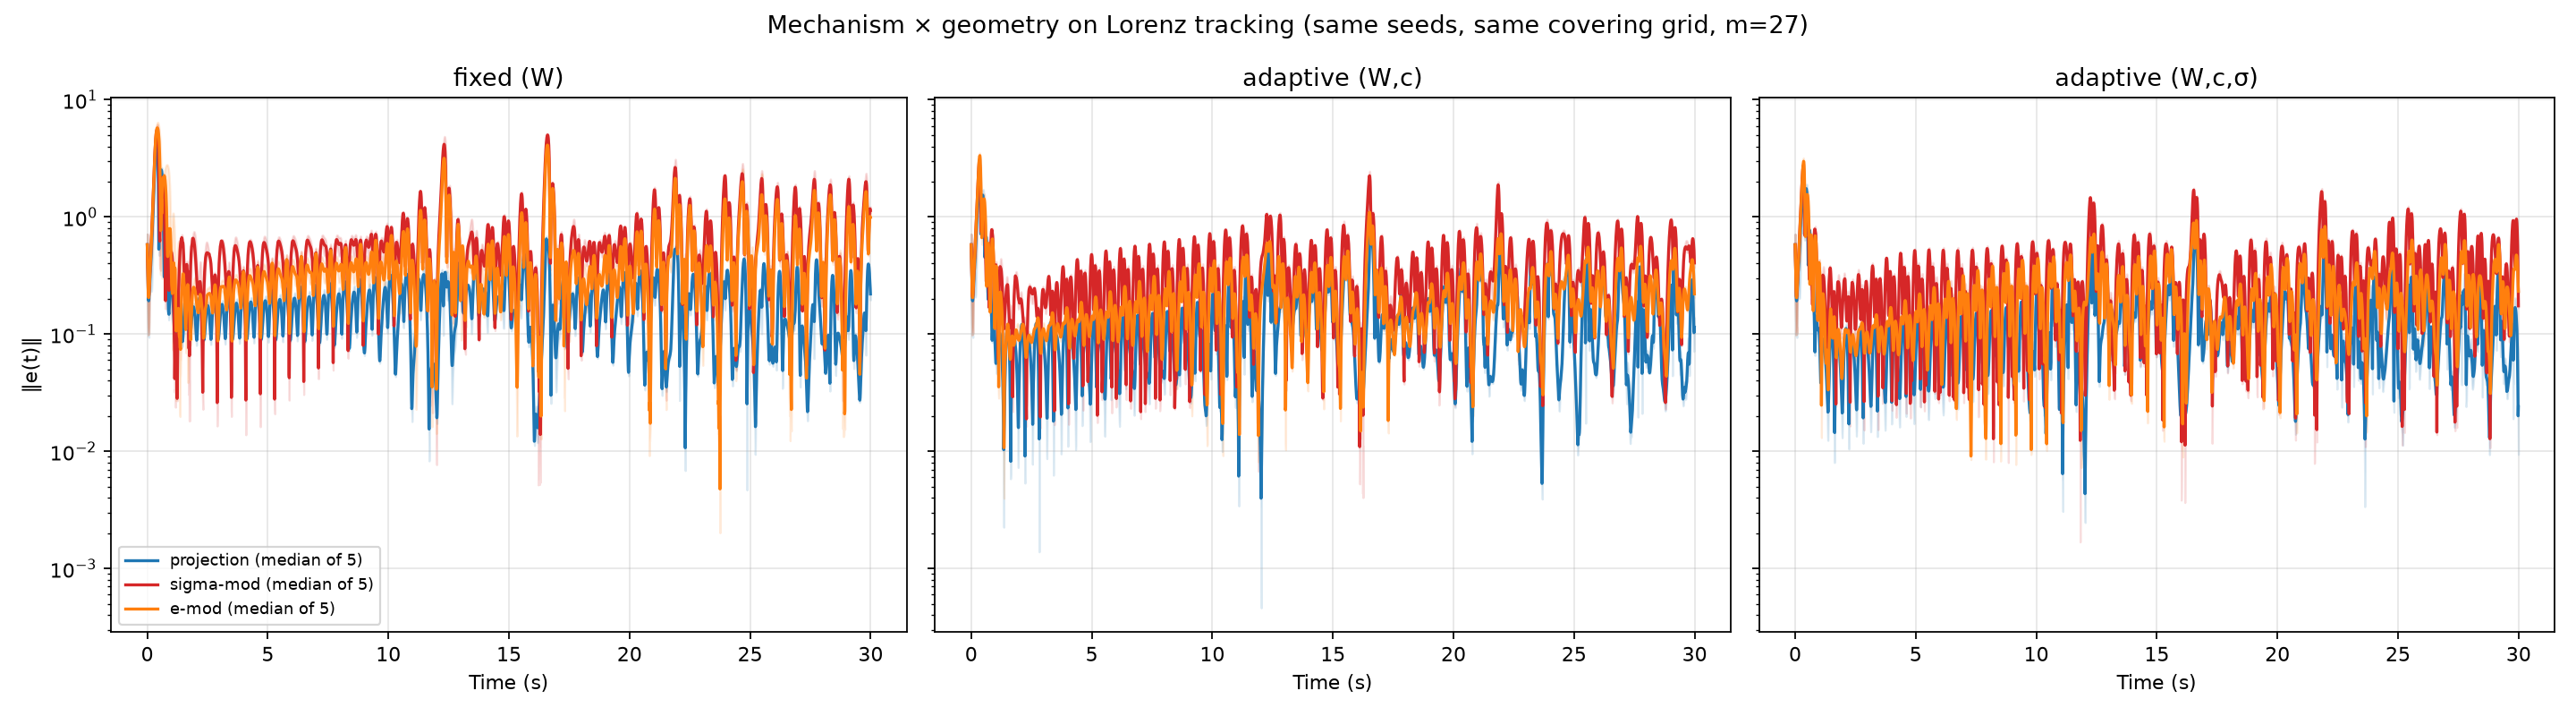
\includegraphics[width=\textwidth]{factorial/figure.png}
\caption[Mechanism $\times$ geometry on Lorenz tracking]{Mechanism $\times$ geometry on Lorenz tracking (same seeds, same covering grid, $m=27$): $\norm{e(t)}$
against time, logarithmic scale, median of the 5 seeds for projection, $\sigma$-modification and $e$-modification;
shaded bands: minimum to maximum over the 5 seeds. Panels: fixed ($W$), adaptive ($W,c$), adaptive ($W,c,\sigma$). Generated by
\code{experiments/exp_bias_factorial.py}.}\label{fig:part1:factorial}
\end{figure}

Projection beats both leaky baselines in every cell, in 5/5 seeds, with paired confidence intervals excluding zero.
Within projection, adaptive centres improve on the fixed grid by $0.0116\pm0.0056$ (5/5 seeds) and adaptive widths
by a further $0.0349\pm0.0026$ (5/5 seeds). So the method's real advantage is the robustness mechanism, with geometry
adaptation a smaller second-order gain --- close to the reverse of the story told by the original headline figure.

\subsection{Kernel-regression baselines}

Table~\ref{tab:part1:complete} is the comparison against kernel-regression baselines from saved single runs, with
nothing excluded (in particular the benchmark $n=3$ and the NTK baseline are included). The proposed method is never
first: it ranks 3/5, 2/5, 3/5 and 2/5 at $n=1,2,3,6$. NTK is first at $n=2$ and $n=6$ (mean steady-state $\norm{e}$
0.0015 and 0.0013, against 0.0372 and 0.0044 for the proposed method), and the sparse GP is first at $n=3$ (3.2729),
where the error of the proposed method is 7.7190. Its genuine edge is cost against the GP baselines: the mean update
time of the proposed method is 0.10, 0.22 and 0.60\,ms per step at $n=1,2,6$ and 4.11\,ms at $n=3$, against
52.92--1888.80\,ms per update for the GP baselines, which update every 50--100 steps. NTK takes 1.59--13.22\,ms per
update; it updates every 50 steps at $n=1$ and every step at $n=2,3,6$ (\code{experiments/sim4_ntk_control.py},
\code{experiments/sim4_ntk_n2.py}, \code{experiments/sim4_ntk_n3.py}, \code{experiments/sim4_ntk_n6.py}), so it is
cheaper than the proposed method only at $n=3$ (2.35 against 4.11\,ms per step). The comparison is not
information-matched: every baseline, here and in the fair re-run below, is trained on noise-free samples of the true
$f(x,t)$, which amounts to measuring the state derivative exactly, whereas the adaptive law uses only the tracking
error $e$. With one run per cell no valid
significance test is available.

\begin{table}[htbp]
\centering\small
\caption[Higher-dimensional comparison, complete]{Higher-dimensional comparison, complete (nothing excluded). Single trajectory per cell; steady state = last
40\% of 30\,s. Step time = mean wall-clock time of the method's update call (GP: per update, every 50--100 steps;
NTK: per update, every 50 steps at $n=1$ and every step at $n=2,3,6$; proposed: per step). No valid significance test
is available (one run per cell). Generated by \code{experiments/plot_comparison_hd_complete.py}; source:
\code{results/comparison_complete_table.md}.}\label{tab:part1:complete}
\begin{tabular}{@{}llrrrcr@{}}
\toprule
benchmark & method & \begin{tabular}[b]{@{}r@{}}mean\\SS $\norm{e}$\end{tabular}
  & \begin{tabular}[b]{@{}r@{}}median\\SS\end{tabular} & \begin{tabular}[b]{@{}r@{}}max\\SS\end{tabular}
  & \begin{tabular}[b]{@{}c@{}}rank\\(mean SS)\end{tabular}
  & \begin{tabular}[b]{@{}r@{}}mean update\\time (ms)\end{tabular}\\
\midrule
$n=1$ (1-D plant, & Proposed (Proj) & 0.2342 & 0.1496 & 1.290 & 3/5 & 0.10\\
\quad Lorenz ref.) & Exact GP & 0.2206 & 0.1415 & 1.016 & 1/5 & 273.78\\
 & Sparse GP & 0.2285 & 0.1914 & 0.874 & 2/5 & 52.92\\
 & Deep GP & 0.3963 & 0.2994 & 1.436 & 4/5 & 94.34\\
 & NTK & 0.4286 & 0.3318 & 1.324 & 5/5 & 13.22\\
\addlinespace
$n=2$ & Proposed (Proj) & 0.0372 & 0.0137 & 0.310 & 2/5 & 0.22\\
\quad (Van der Pol) & Exact GP & 0.0555 & 0.0370 & 0.278 & 3/5 & 498.50\\
 & Sparse GP & 0.1771 & 0.0929 & 0.886 & 5/5 & 150.30\\
 & Deep GP & 0.1758 & 0.1169 & 1.097 & 4/5 & 415.37\\
 & NTK & 0.0015 & 0.0009 & 0.006 & 1/5 & 1.59\\
\addlinespace
$n=3$ & Proposed (Proj) & 7.7190 & 5.7197 & 30.476 & 3/5 & 4.11\\
\quad (Lorenz plant) & Exact GP & 10.2774 & 8.8437 & 34.467 & 5/5 & 1888.80\\
 & Sparse GP & 3.2729 & 2.5099 & 19.176 & 1/5 & 264.64\\
 & Deep GP & 9.5344 & 8.3305 & 33.755 & 4/5 & 802.93\\
 & NTK & 5.7642 & 4.2944 & 18.240 & 2/5 & 2.35\\
\addlinespace
$n=6$ & Proposed (Proj) & 0.0044 & 0.0013 & 0.026 & 2/5 & 0.60\\
\quad (coupled Duffing) & Exact GP & 0.0841 & 0.0695 & 0.279 & 3/5 & 668.01\\
 & Sparse GP & 0.1444 & 0.0872 & 0.670 & 5/5 & 523.83\\
 & Deep GP & 0.0953 & 0.0553 & 0.342 & 4/5 & 1607.48\\
 & NTK & 0.0013 & 0.0010 & 0.004 & 1/5 & 4.75\\
\bottomrule
\end{tabular}
\end{table}

In the original baseline scripts (\code{sim1}--\code{sim3}) the GP baselines held a stale prediction for 50--100 steps,
and the inducing points of the sparse GP lay on a diagonal line over $x\in[-3,3]$ while the reference spans $\pm20$.
The fair re-run at $n=1$ (\code{experiments/kernel_baselines_fair.py}, \code{experiments/run_fair_n1.py},
\code{experiments/plot_fair_n1.py}) uses per-step prediction for all methods, a covering inducing grid and 3 seeds
(Table~\ref{tab:part1:fair}, Figure~\ref{fig:part1:fair}). The mean steady-state $\norm{e}$ is 0.0591 for the exact
GP, 0.1867 for the sparse GP, 0.1978 for the proposed method, 0.3087 for the deep GP and 0.4700 for NTK; the median
online step is 6.309, 1.353, 0.060, 4.461 and 0.212\,ms respectively. Once it is allowed to predict every step, the
exact GP is 3--4$\times$ more accurate than the proposed method (mean steady-state $\norm{e}$ 0.0591 against 0.1978),
and more accurate in every seed (the proposed method has the lower mean in 0/3 seeds). The proposed method is on par
with a fixed-grid sparse GP (the proposed method has the lower mean in 2/3 seeds) at $22.6\times$ lower cost (median
step 0.060\,ms against 1.353\,ms); its step is the cheapest of the five methods. This is the version of the comparison to quote.

\begin{table}[htbp]
\centering\small
\caption[Fair 1-D kernel comparison]{Fair 1-D kernel comparison: per-step prediction for every method, covering inducing grid, seed-level
statistics. Seeds: 3 (different reference and plant initial conditions). Steady state = last 40\% of 30\,s. Step time
= median full online step (prediction + amortised training) after warm-up, same process type, 2 BLAS threads.
Source: \code{results/fair_n1/table.md}.}\label{tab:part1:fair}
\begin{tabular}{@{}lcrrrc@{}}
\toprule
method & \begin{tabular}[b]{@{}c@{}}mean SS $\norm{e}$\\(mean $\pm$ 95\% CI\\over seeds)\end{tabular}
  & \begin{tabular}[b]{@{}r@{}}max SS $\norm{e}$\\(mean)\end{tabular}
  & \begin{tabular}[b]{@{}r@{}}median\\step (ms)\end{tabular}
  & \begin{tabular}[b]{@{}r@{}}mean\\step (ms)\end{tabular}
  & \begin{tabular}[b]{@{}c@{}}seeds where\\proposed has\\lower mean SS\end{tabular}\\
\midrule
Proposed (Proj) & $0.1978\pm0.0503$ & 1.147 & 0.060 & 0.069 & ---\\
Exact GP & $0.0591\pm0.0061$ & 0.780 & 6.309 & 13.936 & 0/3\\
Sparse GP ($9\times3$ grid) & $0.1867\pm0.0210$ & 0.699 & 1.353 & 2.732 & 2/3\\
Deep GP & $0.3087\pm0.1121$ & 1.262 & 4.461 & 5.495 & 2/3\\
NTK & $0.4700\pm0.0250$ & 1.438 & 0.212 & 0.503 & 3/3\\
\bottomrule
\end{tabular}
\end{table}

\begin{figure}[htbp]
\centering
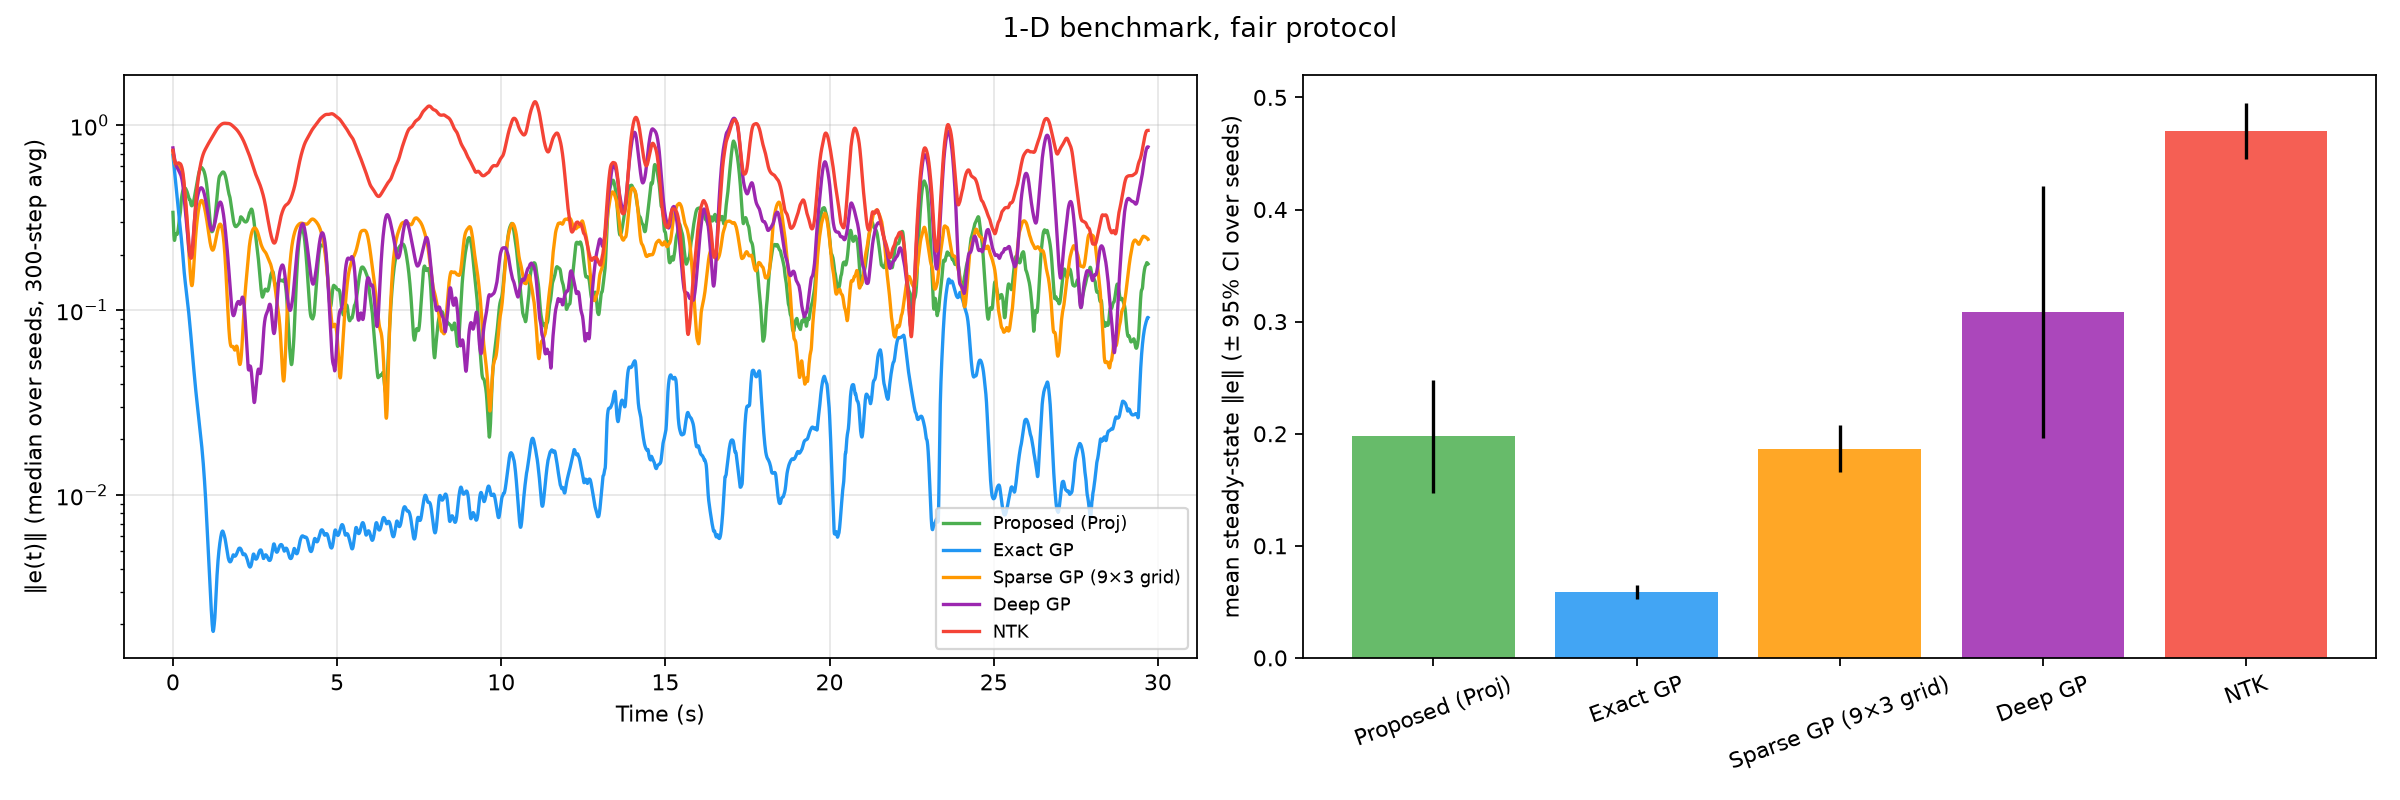
\includegraphics[width=\textwidth]{fair_n1/figure.png}
\caption[1-D benchmark, fair protocol]{1-D benchmark, fair protocol. Left: $\norm{e(t)}$ (median over seeds, 300-step average), logarithmic scale,
for the proposed method (Proj), the exact GP, the sparse GP ($9\times3$ grid), the deep GP and NTK. Right: mean
steady-state $\norm{e}$ ($\pm$ 95\% CI over seeds). Generated by \code{experiments/plot_fair_n1.py}; numbers in
Table~\ref{tab:part1:fair}.}\label{fig:part1:fair}
\end{figure}

\subsection{The bound against data}

\paragraph{Oracle bound study.} The oracle experiment (\code{experiments/exp_oracle_ruub.py}) uses a plant that is
exactly representable with constant $\theta^*$ ($m=8$, $n=2$), so every constant of Theorem~1 is computable; with $\theta^*$ constant,
$C_\Omega=0$ and $R_{\mathrm{UUB}}=D_{\max}/k_e$, reported as $D_{\mathrm{theory}}/k_e$ with $D_{\max}$ from Lemma~2.
The ``full-state bound'' is $\sqrt{R_{\mathrm{UUB}}^2+2V_{\max,\Theta}}$ of Theorem~1(ii), and $D_{\mathrm{meas}}$ is
the measured $\sup_{t\in[10,30]}\norm{d(t)}$ over the evaluation window. Table~\ref{tab:part1:oracle} and
Figure~\ref{fig:part1:oracle} cover $k_e\in\{2,5,10,20\}$ and four learning-rate scales, 3 seeds each. The Lyapunov
identity of Lemma~3 holds to $3.55\times10^{-15}$ (maximal $\abs{\dot V-(-k_e\norm{e}^2+e^\T d+\mathrm{cross})}$),
property (P) is never violated, the hard bounds held, and the RMS bound of Theorem~1(iii) with the measured
disturbance holds in 48/48 runs and tracks $1/k_e$. The a-priori $R_{\mathrm{UUB}}$ is 26.1--261.1 against observed
RMS errors of 0.0087--0.0908; the ratio of the a-priori bound to the observed RMS error ranges from $915\times$ to
$10954\times$.

\begin{table}[htbp]
\centering\footnotesize\setlength{\tabcolsep}{4pt}
\caption[Oracle $R_{\mathrm{UUB}}$ study]{Oracle $R_{\mathrm{UUB}}$ study (exactly representable plant, constant $\theta^*$, $m=8$, $n=2$). Window
$[10,30]$\,s; mean over 3 seeds. All bounds in the same units as $\norm{e}$. ``P viol'' = samples with
$\mathrm{cross}>0$ (must be 0); ``inside'' = hard bounds held. RMS bound (measured disturbance) satisfied in all 48
runs: True. Maximal identity error $\abs{\dot V-(-k_e\norm{e}^2+e^\T d+\mathrm{cross})}$: $3.55\times10^{-15}$.
Source: \code{results/oracle_ruub/table.md}.}\label{tab:part1:oracle}
\begin{tabular}{@{}rrrrrrrrrcc@{}}
\toprule
$k_e$ & \begin{tabular}[b]{@{}r@{}}$\Gamma$\\scale\end{tabular}
  & \begin{tabular}[b]{@{}r@{}}RMS\\$\norm{e}$\end{tabular}
  & \begin{tabular}[b]{@{}r@{}}max SS\\$\norm{e}$\end{tabular}
  & \begin{tabular}[b]{@{}r@{}}RMS bound\\($D_{\mathrm{meas}}$,\\finite window)\end{tabular}
  & $D_{\mathrm{meas}}/k_e$ & $D_{\mathrm{theory}}/k_e$
  & \begin{tabular}[b]{@{}r@{}}full-state\\bound\end{tabular}
  & \begin{tabular}[b]{@{}r@{}}ratio\\theory/RMS\end{tabular}
  & \begin{tabular}[b]{@{}c@{}}P\\viol\end{tabular} & inside\\
\midrule
2 & 0.5 & 0.0908 & 0.1704 & 0.6791 & 0.5435 & 261.1 & 261.9 & 2875$\times$ & 0 & True\\
2 & 1 & 0.0616 & 0.1215 & 0.6801 & 0.6123 & 261.1 & 261.5 & 4239$\times$ & 0 & True\\
2 & 2 & 0.0383 & 0.0796 & 0.7139 & 0.6808 & 261.1 & 261.3 & 6824$\times$ & 0 & True\\
2 & 5 & 0.0238 & 0.0476 & 1.1766 & 1.1649 & 261.1 & 261.2 & 10954$\times$ & 0 & True\\
\addlinespace
5 & 0.5 & 0.0533 & 0.1054 & 0.3170 & 0.1979 & 104.4 & 106.4 & 1958$\times$ & 0 & True\\
5 & 1 & 0.0392 & 0.0708 & 0.2793 & 0.2123 & 104.4 & 105.4 & 2664$\times$ & 0 & True\\
5 & 2 & 0.0270 & 0.0539 & 0.2601 & 0.2240 & 104.4 & 104.9 & 3866$\times$ & 0 & True\\
5 & 5 & 0.0157 & 0.0329 & 0.2925 & 0.2780 & 104.4 & 104.6 & 6662$\times$ & 0 & True\\
\addlinespace
10 & 0.5 & 0.0398 & 0.0793 & 0.1970 & 0.0981 & 52.2 & 56.1 & 1313$\times$ & 0 & True\\
10 & 1 & 0.0266 & 0.0519 & 0.1596 & 0.1003 & 52.2 & 54.2 & 1965$\times$ & 0 & True\\
10 & 2 & 0.0194 & 0.0369 & 0.1395 & 0.1057 & 52.2 & 53.2 & 2688$\times$ & 0 & True\\
10 & 5 & 0.0117 & 0.0240 & 0.1335 & 0.1188 & 52.2 & 52.6 & 4466$\times$ & 0 & True\\
\addlinespace
20 & 0.5 & 0.0285 & 0.0522 & 0.1290 & 0.0501 & 26.1 & 33.2 & 915$\times$ & 0 & True\\
20 & 1 & 0.0197 & 0.0389 & 0.0987 & 0.0494 & 26.1 & 29.9 & 1328$\times$ & 0 & True\\
20 & 2 & 0.0132 & 0.0260 & 0.0799 & 0.0503 & 26.1 & 28.0 & 1971$\times$ & 0 & True\\
20 & 5 & 0.0087 & 0.0168 & 0.0676 & 0.0534 & 26.1 & 26.9 & 3011$\times$ & 0 & True\\
\bottomrule
\end{tabular}
\end{table}

\begin{figure}[htbp]
\centering
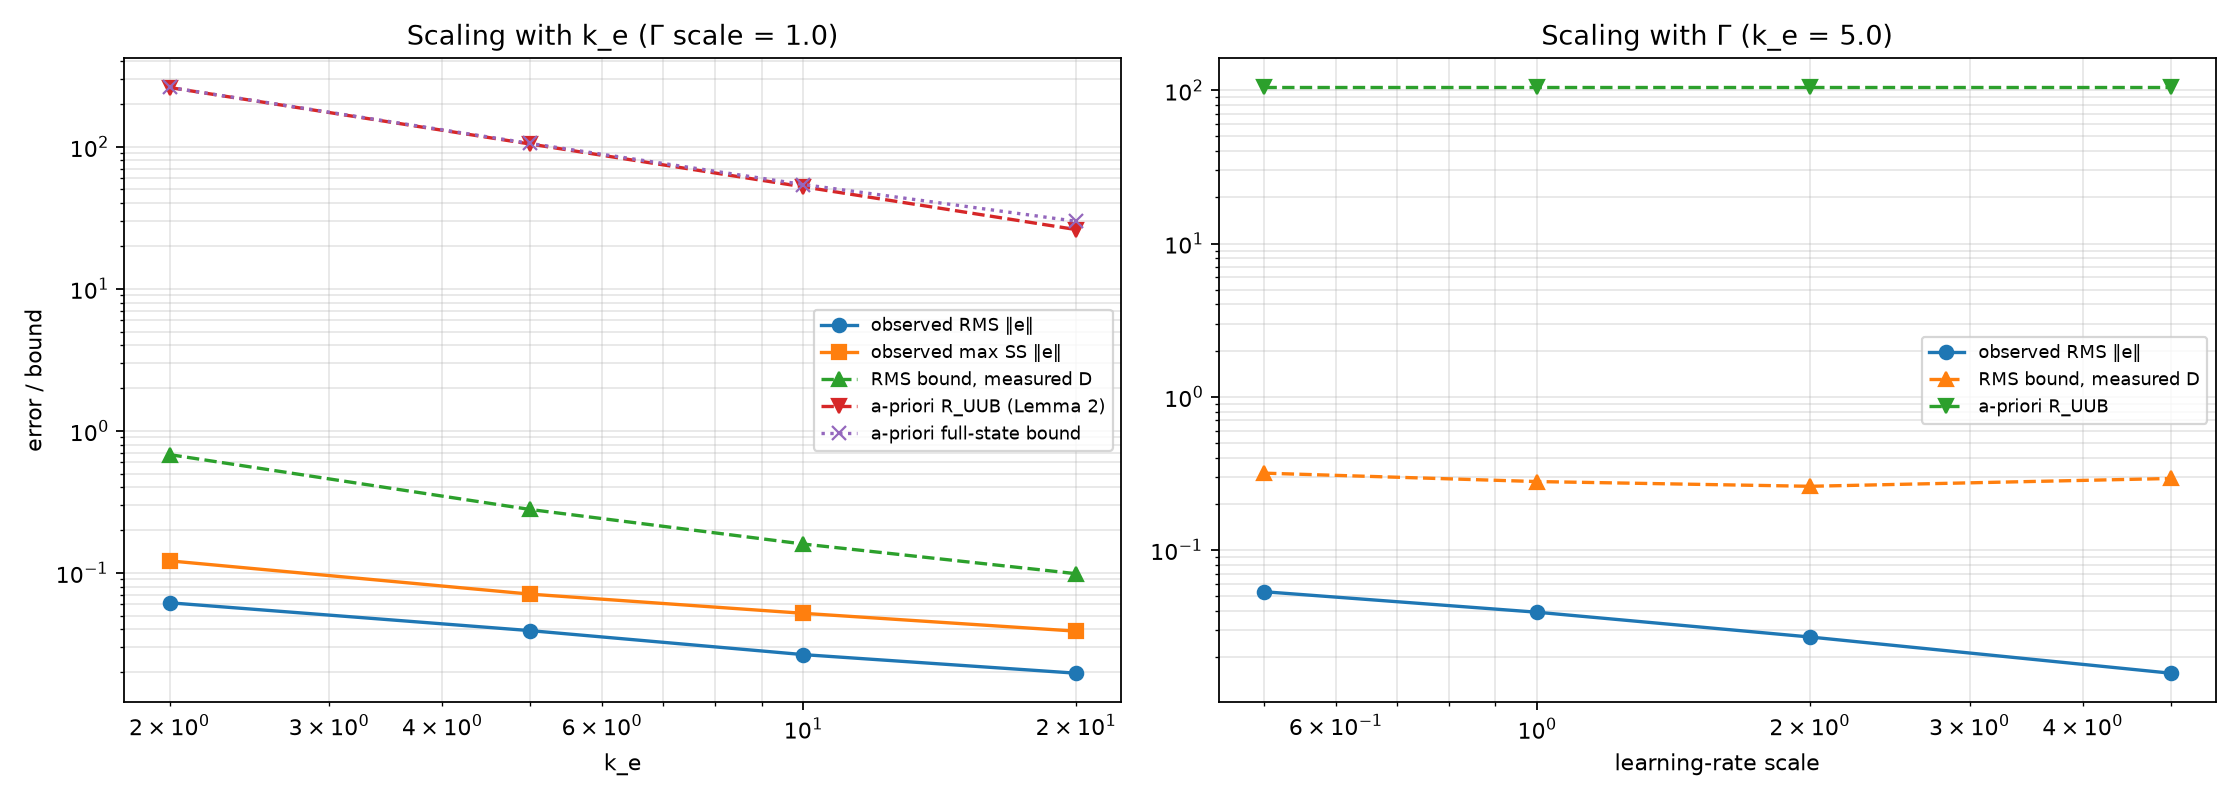
\includegraphics[width=\textwidth]{oracle_ruub/figure.png}
\caption[Oracle bound study]{Oracle bound study, logarithmic axes. Left: scaling with $k_e$ at learning-rate scale 1.0 --- observed RMS
$\norm{e}$, observed maximal steady-state $\norm{e}$, the RMS bound with the measured disturbance, the a-priori
$R_{\mathrm{UUB}}$ (Lemma~2) and the a-priori full-state bound. Right: scaling with the learning-rate scale at $k_e=5$
--- observed RMS $\norm{e}$, the RMS bound with the measured disturbance and the a-priori $R_{\mathrm{UUB}}$. Generated
by \code{experiments/exp_oracle_ruub.py}; numbers in Table~\ref{tab:part1:oracle}.}\label{fig:part1:oracle}
\end{figure}

\begin{table}[htbp]
\centering\small
\caption[Monte Carlo over random initial conditions]{Monte Carlo over random initial conditions (Van der Pol, $m=16$, $k_e=5.0$, 200 trials). Source:
\code{results/monte_carlo_honest/summary.md}.}\label{tab:part1:mc}
\begin{tabularx}{\textwidth}{@{}Yl@{}}
\toprule
check & result\\
\midrule
all trajectories finite & 200/200\\
hard parameter bounds held at every recorded step & 200/200\\
a-posteriori ISS bound
  $\norm{e(t)}\le\mathrm{e}^{-k_e(t-T_1)}\norm{e(T_1)}+\sup\norm{f-\fhat}/k_e$ held & 200/200 (max ratio 0.979)\\
steady-state max $\norm{e}$ (last 25\%): median / 95th pct / max & 0.0568 / 0.0938 / 0.1075\\
steady-state mean $\norm{e}$: median / 95th pct / max & 0.0302 / 0.0484 / 0.0593\\
$\sup\norm{f-\fhat}$ in steady state / $k_e$: median / max & 0.0627 / 0.1475\\
transient max $\norm{e}$: max over trials & 4.903\\
\bottomrule
\end{tabularx}
\end{table}

\paragraph{Monte Carlo over initial conditions.} On a plant that is not exactly representable only exactly checkable
statements are tested (\code{experiments/exp_monte_carlo_honest.py}, Table~\ref{tab:part1:mc}): all 200 trajectories
are finite, the hard parameter bounds held at every recorded step in 200/200 trials, and the a-posteriori ISS bound
held in 200/200 trials (maximal ratio 0.979). No a-priori $R_{\mathrm{UUB}}$ threshold is drawn: $D_{\max}$ and
$C_\Omega$ are not computable for this plant (the threshold 0.5 of the original figure was an arbitrary constant, not a
calculated bound).

\subsection{Summary}

\begin{itemize}
\item On identical geometry, projection beats $\sigma$- and $e$-modification in every cell and in every seed (5/5),
  with paired confidence intervals excluding zero.
\item Adaptive geometry is a smaller but consistent gain: $0.0116$ for adaptive centres and a further $0.0349$ for
  adaptive widths in mean steady-state $\norm{e}$, 5/5 seeds each.
\item Against kernel-regression baselines the proposed method is never the most accurate. Its edge is cost against the
  GP baselines (NTK is cheaper only at $n=3$), and in the fair re-run at $n=1$ it has the cheapest step of the five
  methods.
\item In the fair re-run at $n=1$ the exact GP is 3--4$\times$ more accurate than the proposed method.
\item In the oracle study the a-priori bound exceeds the observed RMS error by factors of $915$ to $10954$, while the
  RMS bound with the measured disturbance holds in 48/48 runs.
\end{itemize}
